\subsection{Market Making}
O market-making é uma forma de negociação (\textit{trading} em inglês) que de forma simplificada consiste em comprar certo ativo a um determinado preço e vender-lo a um preço maior.
Como os preços de compra e venda dos ativos são afetados pela demanda e oferta no momento, cada agente no mercado exerce certa influência sobre o valor de um ativo, a depender das ofertas que o mesmo mantém para tal ativo no livro de ordens limite (\textit{limit order book}, ou \textit{LOB} em inglês). 

No \textit{LOB} os registros se dão primeiramente por ordem de preço, e em segundo por data de criação: as ofertas com melhor preço (tanto para compra como para venda) ficam no topo do livro, e caso tenham o mesmo valor entre si tem sua posição desempatada pela ordem temporal de chegada. No livro de compras, a melhor oferta é a que oferece o maior preço, e o contrário vale para o livro de vendas.

Nas bolsas de valores digitais a execução de uma transação é automática e auxiliada por um sistema chamado de \textit{matching engine} - ou seja, um motor para pareamento de ordens. Esse sistema verifica se para a melhor oferta de compra (ou venda) existe outra correspondente no livro de venda (ou compra) com valor menor ou igual (ou maior ou igual para venda). Após o pareamento, a bolsa anuncia a execução da ordem e as ofertas relacionadas são removidas dos livros.

Em suma, os principais elementos do market making incluem, mas não se limitam à:

\begin{itemize}
	\item Spread: É a diferença entre o preço de compra (\textit{bid} em inglês) e o preço de venda (\textit{ask} em inglês) entre duas ofertas. O market maker busca obter os melhores valores para esses preços, e eventualmente lucrar com a diferença entre eles.
	
	\item Livro de Ordens Limite: É um conjunto ordenado onde as ofertas de compra e venda são registradas. Também é permitido o ajuste dos preços de compra e venda de ofertas existentes por parte dos agentes.
	
	\item Gestão de Risco: Todos \textit{market-makers} enfrentam riscos em suas negociações, entre eles o risco de inventário e risco de mercado. O risco de inventário ocorre quando o \textit{market maker} mantém uma posição desequilibrada entre ativos comprados e vendidos, enquanto o risco de mercado está relacionado às flutuações nos preços dos ativos.
\end{itemize}

No contexto deste projeto, o foco da pesquisa será a otimização de uma estratégia de \textit{market-making} que minimize o risco de inventário durante a noite. A estratégia será composta por um agente responsável pela interação com o mercado e alocação de preços sob políticas para redução de risco. Mais adiante, será apresentado a modelagem do problema como uma cadeia de decisão de Markov. Tendo definido o espaço de ações para o agente e de observações possíveis do mercado, modelaremos a equação de otimalidade de Bellman para os estados do mercado, e discutiremos os algoritmos de Aprendizado por Reforço (RL) que foram escolhidos como abordagem para obter um agente ótimo capaz de aproximar numericamente os preços ótimos.

\subsection{Sistemas dinâmicos e Aprendizado por Reforço}
O Aprendizado por Reforço (RL) é um paradigma de aprendizado baseado em princípios da psicologia comportamental e em otimização estocástica, especificamente tarefas de controle e sistemas dinâmicos. Simplificadamente, trata-se de uma técnica para modelagem, simulação e treino de um agente. Tal agente é capaz de interagir com um ambiente, modelado a partir de um processo de decisão de Markov, com o objetivo de obter uma política de interação com o sistema que maximize sua recompensa cumulativa ao longo do tempo, chamada de "retorno" (note que no contexto de \textit{RL}, o retorno é diferente do 'retorno financeiro' em si).

\begin{figure}[H]
	\centering
	\includegraphics{files/rl-agent.pdf}
	\caption{Autômato do Agente sob o paradigma de Aprendizado por Reforço}
	\label{fig:rl-agent}
\end{figure}

A definição de uma cadeia de decisão com a qual o agente interagirá é uma tupla $MDP = (\mathcal{S}, \mathcal{A}, T_{a}, R_{a})$, onde os elementos que a compõem são:

\begin{description}
	\item[$\mathcal{S}$] 
	é o espaço de estados possíveis, representado por um conjunto onde cada estado $s \in \mathcal{S}$ é uma tupla de $n + 1$ valores numéricos observáveis $s = (x_{0}, x_{1}, \ldots, x_{n})$. Cada estado é uma observação possível da dinâmica do sistema em determinado momento;
	
	\item[$\mathcal{A}$] é o espaço de ações que o agente pode realizar. Uma ação $a \in \mathcal{A}$ é uma tupla com $m + 1$ valores numéricos tal que $a = (y_{0}, y_{1}, \ldots, y_{m})$ são os valores escolhidos pelo agente e aplicados ao sistema, levando à um novo estado.
	
	\item[\textit{T}] é o operador de transição, que representa as transições possíveis entre estado atual $s$ e possível estado futuro $s'$, dado uma ação $a$ tomada pelo agente, tal qual \(T : \mathcal{S} \times \mathcal{A} \times \mathcal{S} \rightarrow [0, 1]\). A função densidade de probabilidade $T$, é tal que $T(s, a, s') = f(s' \,|\, s, a)$ onde $f(s' \,|\, s, a)$ pertence à um espaço de probabilidade qualquer, no intervalo $[0, 1]$.
	
	\item[\textit{R}] é a função de recompensa da cadeia de Markov, que mapeia uma determinada transição (tupla com valores $(s, a, s')$) à recompensa esperada no próximo estado $s'$, tal que
	$R : \mathcal{S} \times \mathcal{A} \times \mathcal{S} \rightarrow \mathbb{R}$, onde $R(s, a, s') = \mathbb{E}[r | s, a, s']$ e $r \sim g(r | s, a, s')$ é a função densidade de recompensa para a transição.
\end{description}

\begin{figure}[H]
	\centering
	\documentclass[tikz,border=10pt]{standalone}
\usepackage{pgf}
\usepackage{xcolor}
\usetikzlibrary{arrows,automata,positioning}

\definecolor{statecolor}{HTML}{e89a6f} 
\definecolor{actioncolor}{HTML}{bcd35f} 

\tikzset{
    state/.style={
        shape=rectangle,
        draw=black,
        fill=statecolor,
        align=center,
        minimum height=2em,
        minimum width=4em,
        inner sep=2pt
    },
    action/.style={
        shape=rectangle,
        draw=black,
        fill=actioncolor,
        align=center,
        inner sep=10pt,
        rounded corners=15pt,
    },
    reward/.style={
    	|->,
    	decoration={snake, amplitude=1.5mm, segment length=3mm},
    	decorate,
    	postaction={draw, line width=1pt, shorten <=1pt, -{Stealth[scale=1.5]}}
    },
    transition/.style={
    	->,
    }
}

\begin{document}
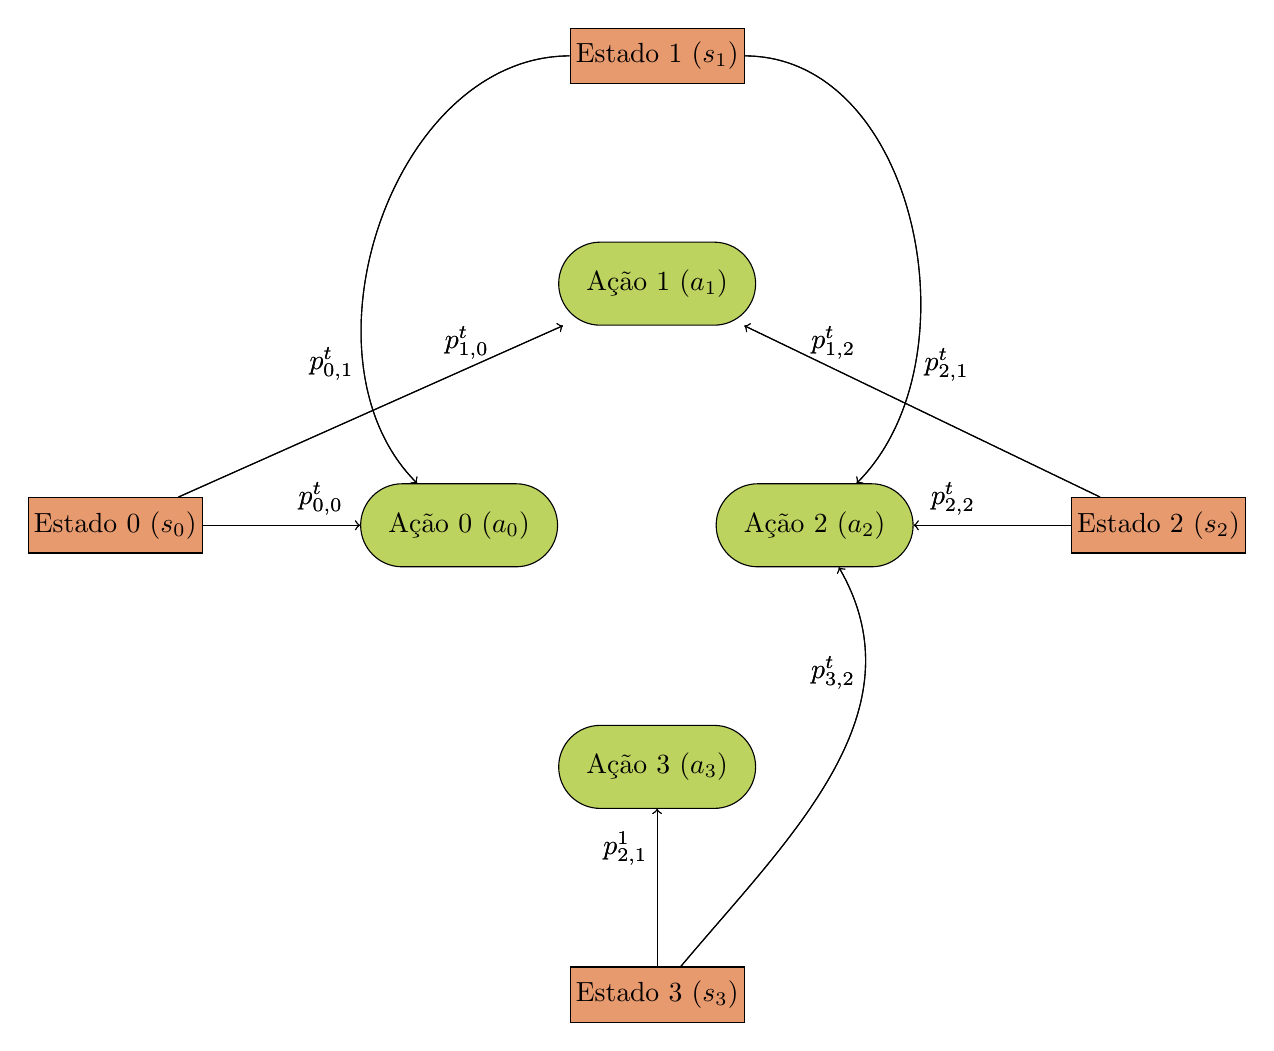
\begin{tikzpicture}
    \node[state] (s0) {Estado 0 ($s_0$)};
    
    \node[action, right=2cm of s0] (a0) {Ação 0 ($a_0$)};
    \node[action, above right=2cm and 0cm of a0] (a1) {Ação 1 ($a_1$)};
    \node[action, right=2cm of a0] (a2) {Ação 2 ($a_2$)};
    \node[action, below right=2cm and 0cm of a0] (a3) {Ação 3 ($a_3$)};
    
    \node[state, above=2cm of a1] (s1) {Estado 1 ($s_1$)};
    \node[state, right=2cm of a2] (s2) {Estado 2 ($s_2$)};
    \node[state, below=2cm of a3] (s3) {Estado 3 ($s_3$)};
    
    \begin{scope} % actions
    	\draw[transition] 
    	(s0) 
    	to node[near end, above] {$p_{0,0}^{t}$} 
    	(a0);
    	
    	\draw[transition] 
    	(s0) 
    	to node[near end, above] {$p_{1,0}^{t}$} 
    	(a1);
    	
    	\draw[transition] 
    	(s1) 
    	to[in=45, out=360] node[near end, right] {$p_{2,1}^{t}$} 
    	(a2);
    	
    	\draw[transition] 
    	(s1) 
    	to[in=135, out=180] node[near end, left] {$p_{0,1}^{t}$} 
    	(a0);
    	
    	\draw[transition] 
    	(s2) 
    	to node[near end, above] {$p_{1,2}^{t}$} 
    	(a1);
    	
    	\draw[transition] 
    	(s2) 
    	to node[near end, above] {$p_{2,2}^{t}$} 
    	(a2);
    	
    	\draw[transition] 
    	(s3) 
    	to node[near end, left] {$p_{2,1}^{1}$} 
    	(a3);
    	
    	\draw[transition] 
    	(s3) 
    	to[in=300, out=50] node[near end, left] {$p_{3,2}^{t}$} 
    	(a2);
    \end{scope}
    \begin{scope} % rewards
    	\draw[transition] 
    	(s0) 
    	to node[near end, above] {$p_{0,0}^{t}$} 
    	(a0);
    	
    	\draw[transition] 
    	(s0) 
    	to node[near end, above] {$p_{1,0}^{t}$} 
    	(a1);
    	
    	\draw[transition] 
    	(s1) 
    	to[in=45, out=360] node[near end, right] {$p_{2,1}^{t}$} 
    	(a2);
    	
    	\draw[transition] 
    	(s1) 
    	to[in=135, out=180] node[near end, left] {$p_{0,1}^{t}$} 
    	(a0);
    	
    	\draw[transition] 
    	(s2) 
    	to node[near end, above] {$p_{1,2}^{t}$} 
    	(a1);
    	
    	\draw[transition] 
    	(s2) 
    	to node[near end, above] {$p_{2,2}^{t}$} 
    	(a2);
    	
    	\draw[transition] 
    	(s3) 
    	to node[near end, left] {$p_{2,1}^{1}$} 
    	(a3);
    	
    	\draw[transition] 
    	(s3) 
    	to[in=300, out=50] node[near end, left] {$p_{3,2}^{t}$} 
    	(a2);
    \end{scope}
\end{tikzpicture}
\end{document}


	\caption{Processo de Decisão de Markov discreto com 4 estados e 4 ações (MDP)}
	\label{fig:mdp}
\end{figure}

Considerando o contexto de controle estocástico, um agente é efetivamente a política de escolha de ações. Dado um estado atual $s$ a política dá a probabilidade do agente escolher uma ação $a$ e enviar à cadeia tal ação. Uma política estocástica $\pi$ qualquer é representada por:

\begin{equation}
	\begin{aligned}
	\pi(a \,|\, s) = h(a \,|\, s)
	\end{aligned}
\end{equation}
onde $h(a \,|\, s)$ é uma função densidade de probabilidade em cima das ações possíveis.
Por fim, o objetivo do agente é obter uma política ótima que maximize o retorno obtido, que é a soma amortizada das recompensas futuras. Para tal, definimos o tempo atual do ambiente como $t \in \mathbb{N}$, que vai até o final do período de observação $T$, tal que $t \leq T$. Assim, o retorno do agente é obtido pela seguinte expressão:

\begin{equation}
	\begin{aligned}
		G_{t} = \sum_{k=0}^{T - t - 1} \gamma^{k} \cdot R_{t + 1 + k}
	\end{aligned}
\end{equation}

onde $\gamma$ é o fator de amortecimento e $R_t$ é a recompensa que o agente recebe no momento $t$, de acordo com uma função de recompensa $R$, ou seja $R_t = R(s_{t}, a_{t}, s_{t + 1})$ (note que $G_{T} = 0$, dado que não é possível receber recompensas após o término do ambiente).

De modo a obter a política que maximize o retorno do agente, é necessário definir duas equações importantes para o contexto de aprendizado por reforço. A função de valor de estado de Bellman \(V_\pi(s)\) quantifica o retorno cumulativo esperado quando um agente começa no estado \(s\) e segue uma política específica \(\pi\):
\[ 
V^{\pi}(s) = \mathbb{E}_\pi[G_t | S_t = s]
\]
onde \(G_t\) é o retorno no tempo e \(S_t\) é o estado no tempo \(t\).

A função de valor de estado-ação, \(Q^\pi(s, a)\), estende a função de valor do estado ao considerar tanto o estado atual \(s\) quanto uma ação escolhida \(a\):
\[ Q^{\pi}(s, a) = \mathbb{E}_\pi[G_t | S_t = s, A_t = a]\]
onde \(A_t\) é a ação tomada no tempo \(t\).

A equação estado-valor de otimalidade, \(V^*(s)\), representa o retorno cumulativo máximo esperado alcançável a partir do estado \(s\) entre todas as políticas possíveis:
\[ V^*(s) = \max_\pi V^{\pi}(s). \]

Por fim, a política ótima $\pi^*$ é obtida ao selecionar ações que maximizam a função de valor de estado-ação:
\begin{equation}
	\begin{aligned}
		\pi^*(a|s) = \arg\max_a Q^*(s, a)
		\label{eq:objective}
	\end{aligned}
\end{equation}
onde \(Q^*(s, a)\) é a função de valor de estado-ação ótima.

Os valores de $Q^{*}$ não são conhecidos para sistemas mais complexos, assim como não são discretizáveis para problemas com espaços de ação ou estado contínuos. Na próxima seção será discutido as técnicas e metodologias possíveis para se obter os valores da equação de estado ação de otimalidade, assim como a necessidade do uso do aprendizado por reforço devido à complexidade de ambientes como bolsas digitais e livros de ordem limite.

Para sistemas dinâmicos simples, é possível obter a função de valores de ação-estado analiticamente, como proposto em \citep{Avellaneda2008} e \citep{rao2020stochastic} para espaços contínuos. Para sistemas com dinâmicas mais complexas existem também métodos de aproximação numérica presentes na literatura de controle estocástico, como os métodos de programação dinâmica, que consistem em aproximar os valores para as probabilidades de transição da política (\textit{policy-iteration}) ou da função valor (\textit{value-iteration}).

Por fim, para espaços discretos extremamente grandes ou espaços contínuos tanto o uso de soluções analíticas como métodos de programação dinâmica ou tabelas se tornam inviáveis, devido a escala e custo computacional do problema. O paradigma de aprendizado por reforço busca possibilitar a aproximação dos valores de $V$ ou $Q$ de modo que convirja e execute em tempo aceitável.  Dentre as técnicas que foram consideradas estão:
\begin{itemize}
	\item \textbf{Temporal Difference Learning (\textit{TD Learning})}
	\begin{itemize}
		\item O \textit{TD Learning} é uma técnica de aprendizado por reforço que visa aprender a função valor de um estado ou ação de forma incremental com base nas diferenças temporais entre as estimativas sucessivas.
		\item A atualização típica do TD learning para um estado \(s\) é dada por \(V(s) \leftarrow V(s) + \alpha \cdot (R + \gamma \cdot V(s') - V(s))\), onde $R$ é a recompensa imediata, \(\gamma\) é o fator de desconto, \(s'\) é o próximo estado, e \(\alpha\) é a taxa de aprendizado.
	\end{itemize}
	
	\item \textbf{\textit{Q-Learning}}
	\begin{itemize}
		\item O \textit{Q-Learning} é um método de aprendizado por reforço que visa aproximar os valores da função Q, que representa a qualidade de tomar uma ação específica em um determinado estado.
		\item A regra de atualização típica do Q-valor é \(Q(s, a) \leftarrow Q(s, a) + \alpha \cdot (R + \gamma \cdot \max_{a'} Q(s', a') - Q(s, a))\), onde \(s'\) é o próximo estado, \(R\) é a recompensa, \(\gamma\) é o fator de desconto e \(\alpha\) é a taxa de aprendizado.
	\end{itemize}
	
	\item \textbf{\textit{Actor-Critic Learning}}
	
	\begin{itemize}
		\item O AC-learning envolve duas partes principais: o crítico (critic) que avalia as ações, e o ator (actor) que escolhe as ações. O objetivo é otimizar a política do ator com base nas avaliações do crítico.
		\item O crítico aprende uma função de valor como no TD learning, enquanto o ator atualiza a política para maximizar os valores de ação estimados pelo crítico.
	\end{itemize}
	
	\item \textbf{\textit{Deep Q-Learning (DQL)}}
	
	\begin{itemize}
		\item O DQL é uma extensão do Q-Learning que incorpora redes neurais para lidar com espaços de estados e ações contínuos ou de alta dimensionalidade.
		\item A função Q passa a ser aproximada por uma rede neural profunda. O algoritmo utiliza a experiência passada armazenada em um buffer de repetição para realizar atualizações mais estáveis.
		\item A atualização do Q-valor torna-se \(Q(s, a) \leftarrow Q(s, a) + \alpha \cdot (R + \gamma \cdot \max_{a'} Q(s', a'; \theta^-) - Q(s, a; \theta))\), onde \(\theta\) são os parâmetros da rede neural, e \(\theta^-\) representa os parâmetros da rede no passo anterior.
	\end{itemize}
\end{itemize}

Na próxima seção é discutido o processo de decisão de Markov em termos das variáveis de Market-Making, assim como é explicado o passo a passo para treino do agente por aprendizado por reforço.